\section{Embedded control synthesis}
\subsection{Embedded pole-constrained $\mathcal{H}_2$ control}


\begin{frame}{Embedded control synthesis}{Literature: nested PI control \footnote{M. Bodson et al., "\textbf{High-performance non-linear feedback control of a permanent magnet stepper motor}," \textit{IEEE Transactions on Control Systems Technology}, pp. 5–14, 1993.}}
    \vspace{-0.6cm}
    \begin{figure}
        \begin{psfrags}
        \def\textsize{.5}

        \psfrag{Vr}[c][c][\textsize]{\bfseries\color{blue4}$\rho^\#$}
        \psfrag{thm}[c][c][\textsize]{\bfseries\color{blue4}$\theta$}
        \psfrag{wm}[c][c][\textsize]{\bfseries\color{green4}$\omega$}
        \psfrag{iabc}[c][c][\textsize]{\bfseries\color{blue4}$i_{abc}$}
        \psfrag{idq}[c][c][\textsize]{\bfseries\color{blue4}$i_{dq}$}
        \psfrag{vabcr}[c][c][\textsize]{\bfseries\color{blue4}$v_{abc}^\#$}
        \psfrag{vdq2}[c][c][\textsize]{\bfseries\color{blue4}$v_{dq}$}
        \psfrag{dq}[c][c][.5]{\bfseries\color{blue4}${dq}$}
        \psfrag{abc}[c][c][.5]{\bfseries\color{blue4}${abc}\quad$}
        \psfrag{S}[c][c][\textsize]{\bfseries\color{green4}$S_{abc}$}
        \psfrag{ParkInv}[c][c][.5]{}
        \psfrag{Park}[c][c][.5]{}
        \psfrag{ref}[c][c][\textsize]{\bfseries\color{cyan4}$\omega^\#$}

        \psfrag{MLI}[c][c][.4]{\bfseries\color{blue4}Modulation}
        \psfrag{Onduleur}[c][c][\textsize]{\bfseries\color{red4}Inverter}
        \psfrag{PMSM}[c][c][\textsize]{\bfseries\color{red4}PMSM}

        \psfrag{V}[c][c][\textsize]{\bfseries\color{red4}$v_{abc}$}
        \psfrag{th}[c][c][\textsize]{\bfseries\color{red4}$\theta$}
        \psfrag{w}[c][c][\textsize]{\bfseries\color{red4}$\omega$}
        \newcommand{\sat}{\mathrm{sat}}

        \psfrag{Dynamique}[c][c][\textsize]{\bfseries\color{green4}Dynamic}
        \psfrag{Asservissement}[c][c][\textsize]{\bfseries\color{blue4}control}
        \psfrag{Elec}[c][c][\textsize]{\bfseries\color{blue4}Electrical}
        \psfrag{Dynamique2}[c][c][\textsize]{\bfseries\color{blue4}Dynamic}
        \psfrag{Asservissement2}[c][c][\textsize]{\bfseries\color{green4}control}
        \psfrag{Meca}[c][c][\textsize]{\bfseries\color{green4}Mechanical}
        \psfrag{CapW}[c][c][\textsize]{\bfseries\color{green2}Mechanical}

        \psfrag{Idqr2}[c][c][\textsize]{\bfseries\color{green4}$i_{dq}$}
        \psfrag{Idqr}[c][c][\textsize]{\bfseries\color{green4}${i_{dq}^\#}$}
        \psfrag{vdqr}[c][c][\textsize]{\bfseries\color{blue4}$v_{dq}^\#$}
        \psfrag{+r}[c][c][\textsize]{\bfseries\color{red4}$+$}
        \psfrag{-r}[c][c][\textsize]{\bfseries\color{red4}$-$}
        \psfrag{+v}[c][c][\textsize]{\bfseries\color{blue4}$+$}
        \psfrag{-v}[c][c][\textsize]{\bfseries\color{blue4}$-$}
        \psfrag{+b}[c][c][\textsize]{\bfseries\color{green4}$+$}
        \psfrag{-b}[c][c][\textsize]{\bfseries\color{green4}$-$}

        \psfrag{TSM}[l][c][.7]{\bfseries\color{green4}$F_{s,m}= 1$kHz}
        \psfrag{TSE}[l][c][.7]{\bfseries\color{blue4}$F_{s,e}= 20$kHz}

        \psfrag{Embedded}[l][c][1]{\bfseries\color{red}Embedded code}

        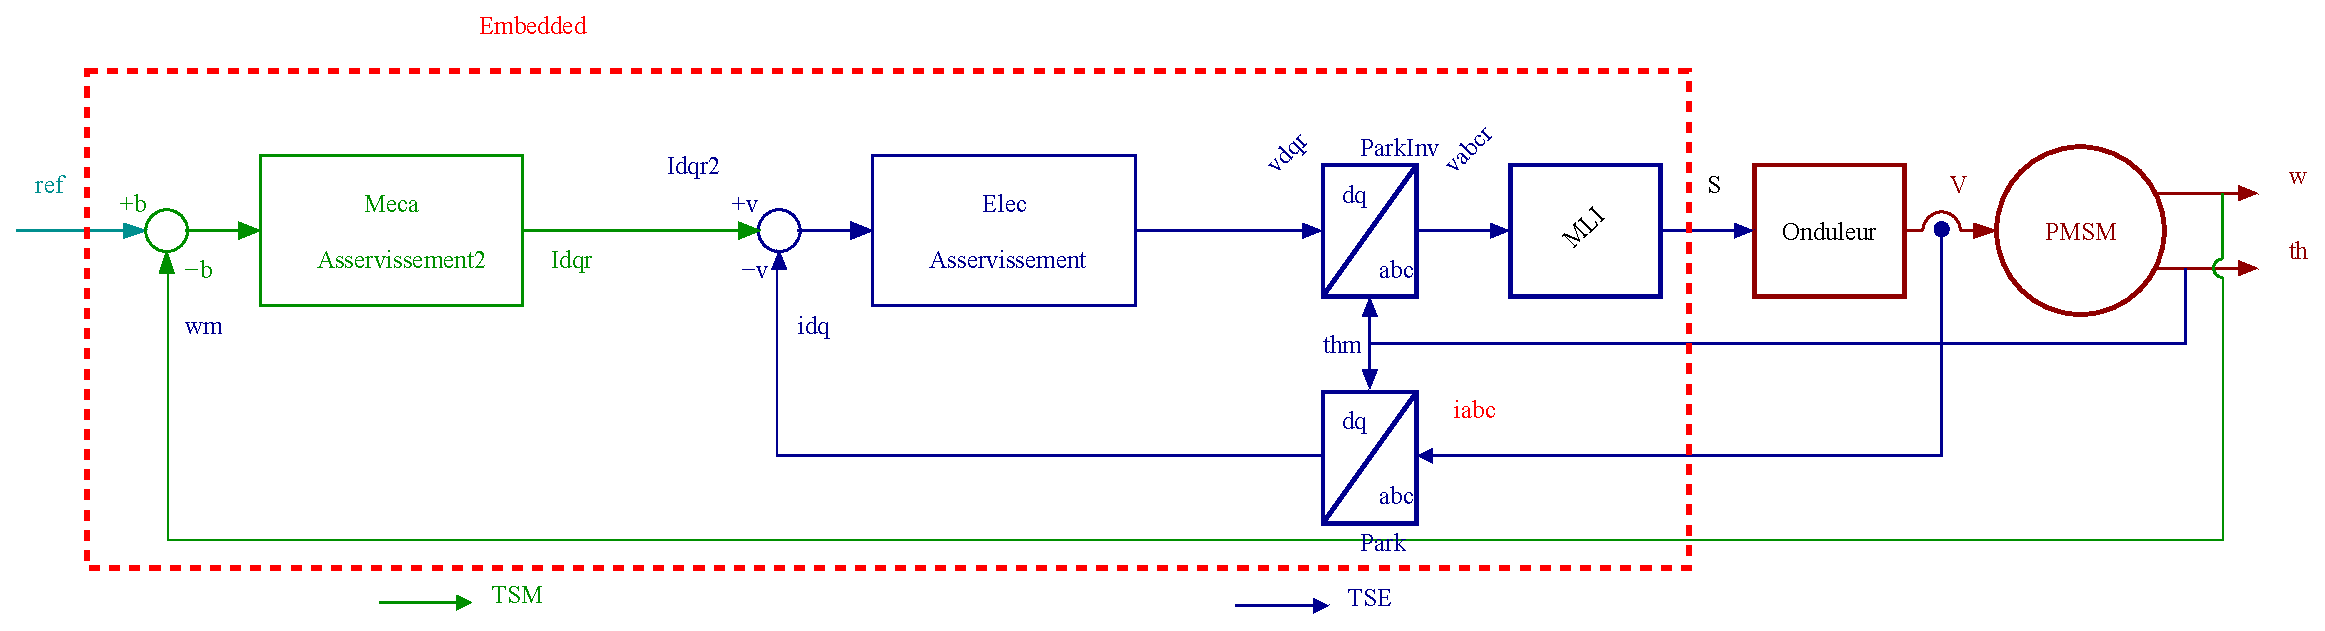
\includegraphics[width = 0.8\textwidth]{pictures/ControlFOC_sanssat.eps}
        \end{psfrags}
\end{figure}

\vspace{0.1cm}
%\begin{columns}[t]
 %   \begin{column}{0.48\textwidth}
        \textbf{Classical approach:}
        \begin{itemize}
            \item Linearize the PMSM model
            \item Second-order  closed-loop dynamics: 
                \begin{itemize}
                    \item Electrical dynamics ($i_d$, $i_q$)
                    \item Mechanical dynamics ($\omega$)
               \end{itemize}
            \item Nested PI controllers
        \end{itemize}
 %   \end{column}

    % \begin{column}{0.48\textwidth}
    %     \textbf{PI characteristics:}
    %     \begin{itemize}
    %           %  \item[\textcolor{blue}{$\checkmark$}] \textcolor{blue}{Hard constraints on poles}
    %             \item[\textcolor{blue}{$\checkmark$}] \textcolor{blue}{Easy to tune $\rightarrow$ hard constraints}
    %             \item[\textcolor{red}{$\times$}] \textcolor{red}{Too restrictive}
    %             \item[\textcolor{red}{$\times$}] \textcolor{red}{No performance optimization}
    %             \item[\textcolor{red}{$\times$}] \textcolor{red}{Difficult to explicitly guarantee robustness}
    %     \end{itemize}
    % \end{column}
%\end{columns}

\end{frame}

\begin{frame}{Embedded control synthesis}{Control synthesis challenges \footnote{ B. Stellato et al., "\textbf{OSQP: an operator splitting solver for quadratic programs}," \textit{Mathematical Programming Computation}, vol. 12, no. 4, pp. 637--672, \textbf{2020}.}}

    \vspace{0.2cm}
    \begin{columns}[t]
        \begin{column}{0.5\textwidth}
            \textbf{PI controllers:}
            \begin{itemize}
                \item[\textcolor{blue}{$\checkmark$}] \textcolor{blue}{Easy to tune: relate $t_r$, overshoot to eigenvalues}
                \item[\textcolor{blue}{$\checkmark$}] \textcolor{blue}{Specific pole locations}
                \item[\textcolor{red}{$\times$}] \textcolor{red}{Too restrictive: no performance optimization}
            \end{itemize}
            \vspace{-0.1cm}
            \centering
            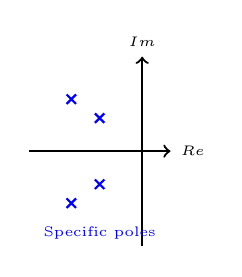
\begin{tikzpicture}[scale=1.2]
                \def\xmin{-1.2cm} \def\xmax{0.3cm}
                \def\ymin{-1.0cm} \def\ymax{1.0cm}

                \draw [thick,->] (\xmin,0) -- (\xmax,0) node [anchor = west]{\tiny $\operatorname{Re}$};
                \draw [thick,->] (0,\ymin) -- (0,\ymax) node [anchor = south]{\tiny $\operatorname{Im}$};

                % Draw crosses for specific eigenvalue locations
                \draw[blue, thick] (-0.5,0.3) -- (-0.4,0.4) (-0.5,0.4) -- (-0.4,0.3);
                \draw[blue, thick] (-0.5,-0.3) -- (-0.4,-0.4) (-0.5,-0.4) -- (-0.4,-0.3);
                \draw[blue, thick] (-0.8,0.5) -- (-0.7,0.6) (-0.8,0.6) -- (-0.7,0.5);
                \draw[blue, thick] (-0.8,-0.5) -- (-0.7,-0.6) (-0.8,-0.6) -- (-0.7,-0.5);

                \node[blue, below] at (-0.45,-0.7) {\tiny Specific poles};
            \end{tikzpicture}
        \end{column}

        \begin{column}{0.5\textwidth}
            \pause
            \textbf{LQR/MPC:}
            \begin{itemize}
                \item[\textcolor{blue}{$\checkmark$}] \textcolor{blue}{Soft constraints $ \min \int_0^\infty (x^\top Q x + u^\top R u) dt$}
                \item[\textcolor{red}{$\times$}] \textcolor{red}{Difficult to tune $Q$, $R$}
                \item[\textcolor{red}{$\times$}] \textcolor{red}{Difficult to explicitly guarantee robustness}
            \end{itemize}
            \vspace{+0.5cm}
                    
        \textbf{Note:} Both methods already embedded in microcontrollers
        \end{column}

    \end{columns}
    %
\end{frame}

\begin{frame}{Embedded control synthesis}{Pole-constrained $\mathcal{H}_2$ control via LMI}
For the same linearized model: 

\vspace{+0.1cm} \textbf{Goal:} \textcolor{blue}{\textbf{Both hard and soft constraints}} + robustness

    \vspace{0.4cm}
    \begin{columns}[t]
    \begin{column}{0.45\textwidth}
        %%%%%%%%% LMI regions figure
    \begin{figure}[]
        \centering
        \begin{tikzpicture}[scale=1.8]
    \def\xmin{-1.4cm} \def\xmax{0.5cm}
    \def\ymin{-1.4cm} \def\ymax{1cm}

    \draw [thick,->] (\xmin,0) -- (\xmax,0) node [anchor = west]{$\operatorname{Re}(z)$};
    \draw [thick,->] (0,\ymin) -- (0,\ymax) node [anchor = south]{$\operatorname{Im}(z)$};
    \begin{scope}
      \clip (-1cm,-1cm) rectangle (-0.3cm,1cm);
      \fill[gray!30,opacity=0.6] (-0.3cm,0.3cm) -- (-0.3cm,-0.3cm) -- (-1cm,-1cm) -- (-1cm,1cm) -- cycle;
    \end{scope}
    \draw [darkGreen,line width= 0.4mm] (-0.3cm,-0.3cm) -- (-0.3cm,0.3cm);
    \draw [darkGreen,line width= 0.4mm,dashed] (-0.3cm,0.3cm) -- (-0.3cm,1cm);
    \draw [darkGreen,line width= 0.4mm,dashed] (-0.3cm,-0.3cm) -- (-0.3cm,-1cm);
    \draw [darkBlue,line width= 0.4mm, dashed] (0cm,0cm) -- (-0.3cm,0.3cm);
    \draw [darkBlue,line width= 0.4mm] (-0.3cm,0.3cm) -- (-1cm,1cm);
    \draw [darkBlue,line width= 0.4mm, dashed] (-1cm,1cm) -- (-1cm,1cm) node [pos=1,above left] {$\beta$};
    \draw [darkBlue,line width= 0.4mm, dashed] (0cm,0cm) -- (-0.3cm,-0.3cm);
    \draw [darkBlue,line width= 0.4mm] (-0.3cm,-0.3cm) -- (-1cm,-1cm);
    \draw[->,darkBlue] (-0.15,0.15) arc[start angle=145, end angle=175, radius=0.25cm];
    \node[text=darkBlue] at (-0.25,0.15) {\footnotesize $\psi$};
    \draw[<->,darkGreen] (-0.05,-0.9cm) -- (-0.25cm,-0.9cm) node[midway, below, text=darkGreen] { \footnotesize $\alpha$};
        \end{tikzpicture}
    \end{figure}
    \end{column}

    \begin{column}{0.55\textwidth}
    \textbf{Hard constraints:}    \small{(tuning similar to PI controller)}
    \begin{itemize}
        \item \textcolor{darkGreen}{$\mathbb{D}_\alpha$:} $\alpha$ $\rightarrow$ decay rate 
        \item \textcolor{darkBlue}{$\mathbb{D}_\beta$:} $\beta$ $\rightarrow$ damping ratio
    \end{itemize}


    \vspace{0.3cm}
    \textbf{Soft constraint:}    \small{(similar to LQR/MPC cost)}\\
    \begin{equation*}
        \min \int_0^\infty (x^\top Q x + u^\top R u) dt
    \end{equation*}

    Tuning recommendation: $Q = \mathbf{0}$

    \vspace{0.3cm}
    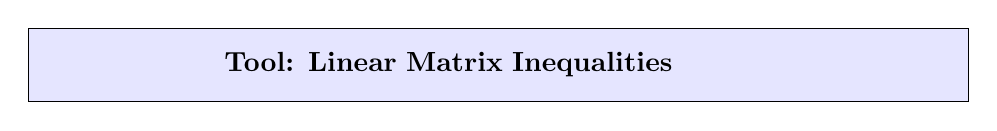
\begin{tikzpicture}
    \node[draw,rectangle,fill=blue!10,text width=0.95\columnwidth,inner sep=6pt]{
    \begin{minipage}{0.9\columnwidth}
    \centering
    \vspace{0.1cm}
    \textbf{Tool: Linear Matrix Inequalities}
    \vspace{0.1cm}
    \end{minipage}};
    \end{tikzpicture}
    \end{column}
    \end{columns}
\end{frame}

\begin{frame}{Embedded control synthesis}{LMI capabilities}

    \begin{columns}[t]
    \begin{column}{0.45\textwidth}
        %%%%%%%%% LMI regions figure with arrow
    \begin{figure}[]
        \centering
        \begin{tikzpicture}[scale=1.8]
    \def\xmin{-1.4cm} \def\xmax{0.5cm}
    \def\ymin{-1.4cm} \def\ymax{1cm}

    \draw [thick,->] (\xmin,0) -- (\xmax,0) node [anchor = west]{$\operatorname{Re}(z)$};
    \draw [thick,->] (0,\ymin) -- (0,\ymax) node [anchor = south]{$\operatorname{Im}(z)$};
    \begin{scope}
      \clip (-1cm,-1cm) rectangle (-0.3cm,1cm);
      \fill[gray!30,opacity=0.6] (-0.3cm,0.3cm) -- (-0.3cm,-0.3cm) -- (-1cm,-1cm) -- (-1cm,1cm) -- cycle;
    \end{scope}
    \draw [darkGreen,line width= 0.4mm] (-0.3cm,-0.3cm) -- (-0.3cm,0.3cm);
    \draw [darkGreen,line width= 0.4mm,dashed] (-0.3cm,0.3cm) -- (-0.3cm,1cm);
    \draw [darkGreen,line width= 0.4mm,dashed] (-0.3cm,-0.3cm) -- (-0.3cm,-1cm);
    \draw [darkBlue,line width= 0.4mm, dashed] (0cm,0cm) -- (-0.3cm,0.3cm);
    \draw [darkBlue,line width= 0.4mm] (-0.3cm,0.3cm) -- (-1cm,1cm);
    \draw [darkBlue,line width= 0.4mm, dashed] (-1cm,1cm) -- (-1cm,1cm) node [pos=1,above left] {$\beta$};
    \draw [darkBlue,line width= 0.4mm, dashed] (0cm,0cm) -- (-0.3cm,-0.3cm);
    \draw [darkBlue,line width= 0.4mm] (-0.3cm,-0.3cm) -- (-1cm,-1cm);
    \draw[->,darkBlue] (-0.15,0.15) arc[start angle=145, end angle=175, radius=0.25cm];
    \node[text=darkBlue] at (-0.25,0.15) {\footnotesize $\psi$};
    \draw[<->,darkGreen] (-0.05,-0.9cm) -- (-0.25cm,-0.9cm) node[midway, below, text=darkGreen] { \footnotesize $\alpha$};

    % Arrow pointing to the gray region from the left
    \draw [->,red,line width=0.6mm] (-1.3cm,0.5cm) -- (-0.6cm,0cm);
    \node[text=red,align=center] at (-1.6cm,0.8cm) {\small Minimize\\[-0.1cm]\small performance\\[-0.1cm]\small criterion};
        \end{tikzpicture}
    \end{figure}
    \end{column}

    \begin{column}{0.55\textwidth}


    %\vspace{0.3cm}
    \textbf{Why LMIs?:}
    %\vspace{0.2cm}
    \begin{itemize}
        \item Convex optimization problems
        \item Hard and soft constraint formulation
        \item Robustness to parametric uncertainty
        \item Anti-windup control design
        \item Formal guarantees via Lyapunov certificates
    \end{itemize}
   
    \end{column}
    \end{columns}

\end{frame}


% \begin{frame}{{Embedded control synthesis}}{PMSM model for pole-constrained $\mathcal{H}_2$ control}
%     %\textbf{LTI state-space form}

%     \begin{columns}[T]
%         \begin{column}{0.5\textwidth}
%             The dynamics of the PMSM is LTI:
%             \begin{align*}
%                 \dot{x}(t) &= Ax(t)+B_u u(t)\\
%                 u(t) &= Kx(t)
%             \end{align*}
%             Augmented with the integral of the tracking error 
%             \begin{eqnarray*}
%                 \varepsilon_{i_d} = \int_{0}^t (i_d^\# - i_d) , d\tau\\
%                 \varepsilon_{\omega} = \int_{0}^t (\omega^\# - \omega) , d\tau\\
%             \end{eqnarray*}
%         \end{column}

%         \begin{column}{0.5\textwidth}
%             \textbf{Control design:}

%             For each subsystem, design $K$ to:
%             \begin{enumerate}
%                 \item Place closed-loop poles in $\mathbb{D}_\alpha \cap \mathbb{D}_\beta$
%                 \begin{itemize}
%                     \item[$\rightarrow$] Transient specifications
%                 \end{itemize}
%                 \item Minimize $\mathcal{H}_2$ norm
%                 \begin{itemize}
%                     \item[$\rightarrow$] Energy efficiency
%                 \end{itemize}
%             \end{enumerate}

%             \vspace{0.3cm}
%             $\Rightarrow$ \textbf{Pole-constrained $\mathcal{H}_2$ synthesis}
%         \end{column}
%     \end{columns}
% \end{frame}


\begin{frame}{Embedded control synthesis}{Pole-constrained $\mathcal{H}_2$ optimization problem}

    % Main content in left minipage
    \begin{minipage}[t]{0.70\textwidth}
    \textbf{Complete LMI formulation:}

    \vspace{-0.2cm}
    \small
    \begin{equation*}
        \min_{X,Y,W,\gamma} \gamma \quad \text{subject to}
    \end{equation*}
    \vspace{-0.3cm}
    \begin{equation*}
        \left.
        \begin{array}{l}
            \begin{bmatrix}
                \langle A\colorbox{SpringGreen}{$X$}+B\colorbox{SpringGreen}{$Y$} \rangle_S  & (*)^\top  \\
                (C_z\colorbox{SpringGreen}{$X$}+D_{z}\colorbox{SpringGreen}{$Y$}) & -I
            \end{bmatrix} \prec 0 \\[3mm]
            \begin{bmatrix}
                \colorbox{SpringGreen}{$W$} & B_w^\top  \\
                B_w & \colorbox{SpringGreen}{$X$}
            \end{bmatrix} \succ 0 \\[3mm]
            \mathrm{trace}(\colorbox{SpringGreen}{$W$}) < \colorbox{SpringGreen}{$\gamma$}
        \end{array}
        \right\} \mathcal{H}_2 \text{ synthesis constraints}
    \end{equation*}
    \vspace{0.2cm}
    \begin{equation*}
        \left.
        \begin{array}{l}
            \langle A\colorbox{SpringGreen}{$X$}+B\colorbox{SpringGreen}{$Y$} \rangle_S  +2 \colorbox{Thistle}{$\alpha$} \colorbox{SpringGreen}{$X$} \prec 0 \\[3mm]
            \begin{bmatrix}
                \colorbox{Thistle}{$\beta$} \langle A\colorbox{SpringGreen}{$X$}+B\colorbox{SpringGreen}{$Y$} \rangle_S  & (*)^\top\\
                (A\colorbox{SpringGreen}{$X$}+B\colorbox{SpringGreen}{$Y$})^\top-(A\colorbox{SpringGreen}{$X$}+B\colorbox{SpringGreen}{$Y$}) & \colorbox{Thistle}{$\beta$} \langle A\colorbox{SpringGreen}{$X$}+B\colorbox{SpringGreen}{$Y$} \rangle_S
            \end{bmatrix} \prec 0
        \end{array}
        \right\} \text{Pole placement constraints}
    \end{equation*}
    \end{minipage}%
    \hfill
    % Small reminder figure in right minipage
    \begin{minipage}[t]{0.27\textwidth}
    \vspace{-1.5cm}
    \hfill
    \begin{tikzpicture}[scale=1.5]
    \def\xmin{-1.4cm} \def\xmax{0.5cm}
    \def\ymin{-1.4cm} \def\ymax{1cm}

    \draw [thick,->] (\xmin,0) -- (\xmax,0) node [anchor = west]{\tiny $\operatorname{Re}$};
    \draw [thick,->] (0,\ymin) -- (0,\ymax) node [anchor = south]{\tiny $\operatorname{Im}$};
    \begin{scope}
      \clip (-1cm,-1cm) rectangle (-0.3cm,1cm);
      \fill[gray!30,opacity=0.6] (-0.3cm,0.3cm) -- (-0.3cm,-0.3cm) -- (-1cm,-1cm) -- (-1cm,1cm) -- cycle;
    \end{scope}
    \draw [darkGreen,line width= 0.3mm] (-0.3cm,-0.3cm) -- (-0.3cm,0.3cm);
    \draw [darkGreen,line width= 0.3mm,dashed] (-0.3cm,0.3cm) -- (-0.3cm,1cm);
    \draw [darkGreen,line width= 0.3mm,dashed] (-0.3cm,-0.3cm) -- (-0.3cm,-1cm);
    \draw [darkBlue,line width= 0.3mm, dashed] (0cm,0cm) -- (-0.3cm,0.3cm);
    \draw [darkBlue,line width= 0.3mm] (-0.3cm,0.3cm) -- (-1cm,1cm);
    \draw [darkBlue,line width= 0.3mm, dashed] (0cm,0cm) -- (-0.3cm,-0.3cm);
    \draw [darkBlue,line width= 0.3mm] (-0.3cm,-0.3cm) -- (-1cm,-1cm);
    % Add labels
    \draw[->,darkBlue] (-0.15,0.15) arc[start angle=145, end angle=175, radius=0.25cm];
    \node[text=darkBlue] at (-0.25,0.15) {\tiny $\psi$};
    \draw[<->,darkGreen] (-0.05,-0.9cm) -- (-0.25cm,-0.9cm) node[midway, below, text=darkGreen] {\tiny $\alpha$};
    \node[text=darkBlue] at (-1cm,1cm) [above left] {\tiny $\beta$};
    % Arrow pointing to the gray region from the left
    \draw [->,red,line width=0.4mm] (-1.3cm,0.5cm) -- (-0.6cm,0cm);
    \node[text=red,align=center] at (-1.6cm,0.8cm) {\tiny Minimize\\[-0.05cm]\tiny performance\\[-0.05cm]\tiny criterion};
    \end{tikzpicture}
    \end{minipage}

\end{frame}
\begin{frame}{Embedded control synthesis}

          % \only<1>{
            
            \begin{figure}
                \centering
                \includegraphics[width=0.7\columnwidth]{pictures/PMSM_test_bench.eps}
            \end{figure}
           %} 
        %    \only<2>{
        %     \vspace{-0.5cm}
        %     \begin{figure}
        %         \centering
        %         \includegraphics[width=0.75\columnwidth]{pictures/combined.eps}
        %     \end{figure}    
        %    }
\end{frame}

\begin{frame}{Embedded control synthesis}{How to solve an LMI problem?}
    \begin{columns}
       \vspace{-1cm} \begin{column}{0.45\textwidth}
            \textbf{Solution methodology:}
            \begin{enumerate}
                \only<1->{\item \textbf{Parametrization}}\only<2>{ : express decision variables as linear combinations of basis matrices
                    \begin{equation*} \label{eq:ParamX}
                         X=  X(\xi) = \sum_{i=1}^{n(n+1)/2} \xi_i X_i
                    \end{equation*}}
                  \only<2->{  The LMI constraints become:
                    \begin{equation*} \label{eq:DefinitionLMI}
                        F(\xi) = F_0 +\sum^{\mu+1}_{i=1}\xi_i F_i \succ 0
                    \end{equation*} }
                \item\only<1->{\textbf{Feasibility}}\only<3>{: find an initial feasible point 
                \begin{equation*} \label{eq:FeasibilityProblem}
                    \begin{aligned}
                    &\underset{\xi= [\xi_e,\gamma],\lambda}{\mathrm{min}} \ \lambda \ \mathrm{s.t.} \\
                    & F(\xi)+\lambda I \succ 0  
                    \end{aligned}
                \end{equation*}}
                \item \only<1->{\textbf{Optimization}}\only<4>{ Minimize the objective function
                 \begin{equation*}\label{eq:optimizationProblem}
                    \begin{aligned}
                    &\underset{\xi= [\xi_e,\gamma],\lambda}{\mathrm{min}} \ \gamma \ \mathrm{s.t.} \\
                    & F(\xi)+\lambda I \succ 0 
                    %& -\varepsilon-\lambda \geq 0 
                    \end{aligned}
                \end{equation*}}
            \end{enumerate}
        \end{column}

        \begin{column}{0.55\textwidth}

            \begin{figure}
                \centering
                \includegraphics[width=0.95\columnwidth]{pictures/combined.eps}
            \end{figure}
        \end{column}
    \end{columns}
\end{frame}

% \begin{frame}{Embedded control synthesis}{Embedded LMI solver}
%     \centering
%     \includegraphics[trim={0cm 0cm 0cm 0cm},clip,width=0.9\framewidth]{pictures/online_offline_ink_trajec_full1.eps}
% \end{frame}

\begin{frame}{Practical implementation: Real-time scheduler}
        \textbf{Hardware platforms:}
    \begin{itemize}
        %\item ATSAME54P20A microcontroller (120 MHz, 256 KB RAM, $\sim$\$5)
        \item dsPIC33AK512 DSC $\sim$\$3
    \end{itemize}
    \textbf{Two concurrent tasks:}
    \vspace{0.2cm}

            \begin{figure}
            \begin{center}
                \def\textsize{.8}
                \psfrag{Algo}[c][c][1]{\color{Blue4}Control}
                \psfrag{Control}[c][c][1]{\color{Blue4}Control}
                \psfrag{iabc}[c][c][\textsize]{\color{Blue4}$i_{abc}$}
                \psfrag{idq}[c][c][\textsize]{\color{Blue4}$i_{dq}$}
                \psfrag{vabcr}[c][c][\textsize]{\color{Blue4}$v_{abc}^\#$}
                \psfrag{vdqr}[c][c][\textsize]{\color{Blue4}$v_{dq}^\#$}
                \psfrag{dq}[c][c][.5]{\color{Blue4}${dq}$}
                \psfrag{abc}[c][c][.5]{\color{Blue4}${abc}\quad$}
                \psfrag{S}[c][c][\textsize]{\color{Blue4}$S_{abc}$}
                \psfrag{MLI}[c][c][\textsize]{\color{Blue4}Mod}
                \psfrag{ParkInv}[c][c][.5]{}
                \psfrag{Park}[c][c][.5]{}
                \psfrag{TS1}[l][c][.6]{\color{Blue4}Higher priority $\approx20$kHz}
                % Reference generation (cyan) - lower priority optimization
                \psfrag{Vr}[c][c][\textsize]{\color{Cyan4}$\rho^\#$}
                \psfrag{ref}[c][c][\textsize]{\color{Cyan4}$\omega^\#$}
                \psfrag{ref2}[c][c][\textsize]{\color{Cyan4}$i_d^\#$}
                \psfrag{ref3}[c][c][\textsize]{\color{Cyan4}$\omega^\#$}
                \psfrag{ref4}[c][c][\textsize]{\color{Cyan4}$i_q$}
                \psfrag{ref5}[c][c][\textsize]{\color{Magenta4} Specification}
                \psfrag{ref6}[c][c][\textsize]{\color{Magenta4} Model}
                \psfrag{Reference}[c][c][\textsize]{\color{Cyan4}Trajectory}
                \psfrag{calculation}[c][c][\textsize]{\color{Cyan4}generation}
                \psfrag{TS2}[l][c][.6]{\color{Cyan4}Lower priority $\approx1$kHz}
                % Embedded synthesis (magenta) - idle task
                \psfrag{Emb}[c][c][\textsize]{\color{Magenta4}Embedded}
                \psfrag{Synt}[c][c][\textsize]{\color{Magenta4}synthesis}
                \psfrag{K}[c][c][\textsize]{\color{Magenta4}K}
                \psfrag{TS3}[l][c][.6]{\color{Magenta4}Idle task}
                % Physical system (red) - PMSM and measurements
                \psfrag{Onduleur}[c][c][\textsize]{\color{Red4}Inverter}
                \psfrag{PMSM}[c][c][\textsize]{\color{Red4}PMSM}
                \psfrag{V}[c][c][\textsize]{\color{Red4}$v_{abc}$}
                \psfrag{th}[c][c][\textsize]{\color{Red4}$\theta$}
                \psfrag{w}[c][c][\textsize]{\color{Red4}$\omega$}
                \psfrag{thm}[c][c][\textsize]{\color{Red4}$\theta$}
                \psfrag{wm}[c][c][\textsize]{\color{Red4}$\omega$}
                \psfrag{Embedded}[l][c][.7]{\color{red}Embedded code}
                \includegraphics[width = .9\textwidth]{pictures/AdvancedControl.eps}
            \end{center}
        \label{fig:AdvencedControlForElectricalMotor}
        \end{figure}
        
   
\end{frame}

\begin{frame}{Embedded control synthesis}{Rate-monotonic scheduler}
    \textbf{Multi-rate scheduling:} High-priority tasks preempt low-priority tasks

    \vspace{0.3cm}
         \begin{figure}
        \centering
        \begin{tikzpicture}[xscale=2, yscale=1, every node/.style={font=\small}]
            % Time line
            \foreach \x in {1,...,4} {
                \draw[gray!50, dashed] (\x,1.3) -- (\x,-2);
            }
            % Gray vertical lines at control task falling edges
            \foreach \x in {1.5,2.0,2.5,3.0,3.5} {
                \draw[gray!50, dashed] (\x,1.3) -- (\x,-2);
            }
            % Double arrow showing sampling period
            \draw[<->,thick,gray] (1.5,-1.75) -- (2.0,-1.75) node[midway,below,gray] {\footnotesize $T_s$};
            \fill[magenta!20] (2,0) -- (2,1) -- (2.4,1) -- (2.4,0) --(2.5,0)--(2.5,1)--(2.8,1)--(2.8,0);
             %%%%%%%%%%%%%%% Pulse high blue
            \foreach \x in {2} {
                \draw[draw= magenta, thick] (\x,0) -- (\x,1) -- (\x+0.8,1) -- (\x+0.8,0);
            }
            %%%%%%%%%%%%%%%% Pulse low blue
            \draw[magenta,thick] (1,0) -- (2,0);
            \draw[magenta,thick] (2.8,0)--(4,0) ;
            \node[align=center, left, magenta, font=\large\bfseries] at (-0.5,0.5) {Embedded \\ LMI solver};
            %%%%%%%%%%%%%%%% Pulse  high red
            \foreach \x in {1.4,1.9,2.4,...,3.4} {
                \draw[thick, blue4, fill=blue4!10] (\x,-1.5) -- (\x,-0.5) -- (\x+0.1,-0.5)-- (\x+0.1,-1.5);
           }
           %%%%%%%%%%%%%%%%% Pulse low red
            \foreach \x in {1,1.5,...,3.5} {
                    \draw[thick, blue4]  (\x,-1.5) -- (\x+0.4,-1.5);
            }
            \node[left, blue4, align=center, font=\large\bfseries] at (-0.5,-1) {Control task};
            %%%%%%%%%%%%%%%%% vertical arrows to explain
            \draw[->,thick] (2,-0.4)--(2,0-0.1);
            \draw[->,thick] (2.4,-0.1) --(2.4,-0.4);
            \draw[->,thick] (2.5,-0.4) --(2.5,-0.1);
            %%%%%%%%%%%%%%%%% Arrow pointing to first rising edge
            \draw[->,thick,magenta] (1.8,1.5) -- (2,1) node[midway,above left,magenta,align=center] {\footnotesize specification or model \\ \footnotesize  change};
            %%%%%%%%%%%%%%%%% Time line
            %\draw[->, thick] (0.5,-1.9) --(4.5,-1.9) node [right, align= center] {time} ;
        \end{tikzpicture}
    \end{figure}

    \vspace{-0.2cm}
    \begin{itemize}
        \item \textcolor{blue4}{High-priority task (20 kHz)}: Control loop runs deterministically
        \item \textcolor{magenta}{Low-priority task (idle)}: LMI solver interrupted when needed
    \end{itemize}
 \end{frame}
% \begin{frame}{Embedded control synthesis}{Experimental validation}
%             \begin{figure}[h!]
%                 \centering 
%                 \centerline{\includegraphics[width=0.7\textwidth]{pictures/PMSM_test_bench.eps}}
%             \end{figure}
% \end{frame}
\begin{frame}{Embedded control synthesis}{Experimental validation}
 \begin{columns}
        \begin{column}{0.5\textwidth}
            \begin{tikzpicture}[scale=1.5]
    \def\xmin{-1.4cm} \def\xmax{0.5cm}
    \def\ymin{-1.4cm} \def\ymax{1cm}

    \draw [thick,->] (\xmin,0) -- (\xmax,0) node [anchor = west]{\tiny $\operatorname{Re}$};
    \draw [thick,->] (0,\ymin) -- (0,\ymax) node [anchor = south]{\tiny $\operatorname{Im}$};
    \begin{scope}
      \clip (-1cm,-1cm) rectangle (-0.3cm,1cm);
      \fill[gray!30,opacity=0.6] (-0.3cm,0.3cm) -- (-0.3cm,-0.3cm) -- (-1cm,-1cm) -- (-1cm,1cm) -- cycle;
    \end{scope}
    \draw [darkGreen,line width= 0.3mm] (-0.3cm,-0.3cm) -- (-0.3cm,0.3cm);
    \draw [darkGreen,line width= 0.3mm,dashed] (-0.3cm,0.3cm) -- (-0.3cm,1cm);
    \draw [darkGreen,line width= 0.3mm,dashed] (-0.3cm,-0.3cm) -- (-0.3cm,-1cm);
    \draw [darkBlue,line width= 0.3mm, dashed] (0cm,0cm) -- (-0.3cm,0.3cm);
    \draw [darkBlue,line width= 0.3mm] (-0.3cm,0.3cm) -- (-1cm,1cm);
    \draw [darkBlue,line width= 0.3mm, dashed] (0cm,0cm) -- (-0.3cm,-0.3cm);
    \draw [darkBlue,line width= 0.3mm] (-0.3cm,-0.3cm) -- (-1cm,-1cm);
    % Add labels
    \draw[->,darkBlue] (-0.15,0.15) arc[start angle=145, end angle=175, radius=0.25cm];
    \node[text=darkBlue] at (-0.25,0.15) {\tiny $\psi$};
    \draw[<->,darkGreen] (-0.05,-0.9cm) -- (-0.25cm,-0.9cm) node[midway, below, text=darkGreen] {\tiny $\alpha$};
    \node[text=darkBlue] at (-1cm,1cm) [above left] {\tiny $\beta$};
    % Arrow pointing to the gray region from the left
    \draw [->,red,line width=0.4mm] (-1.3cm,0.5cm) -- (-0.6cm,0cm);
    \node[text=red,align=center] at (-1.6cm,0.8cm) {\tiny Minimize\\[-0.05cm]\tiny performance\\[-0.05cm]\tiny criterion};
    \end{tikzpicture}
    \end{column}
    \begin{column}{0.5\textwidth}
        
    
            \begin{figure}[h!]
                \centering 
                \centerline{\includegraphics[width=1\columnwidth]{pictures/alpha_step_AK512_1.eps}}
            \end{figure}
\end{column}
\end{columns}
        \end{frame}


\begin{frame}{Embedded control synthesis}{Experimental validation (No laod)}
    \begin{columns}
        \begin{column}{0.4\textwidth}
            \begin{tikzpicture}[scale=1.5]
    \def\xmin{-1.4cm} \def\xmax{0.5cm}
    \def\ymin{-1.4cm} \def\ymax{1cm}

    \draw [thick,->] (\xmin,0) -- (\xmax,0) node [anchor = west]{\tiny $\operatorname{Re}$};
    \draw [thick,->] (0,\ymin) -- (0,\ymax) node [anchor = south]{\tiny $\operatorname{Im}$};
    \begin{scope}
      \clip (-1cm,-1cm) rectangle (-0.3cm,1cm);
      \fill[gray!30,opacity=0.6] (-0.3cm,0.3cm) -- (-0.3cm,-0.3cm) -- (-1cm,-1cm) -- (-1cm,1cm) -- cycle;
    \end{scope}
    \draw [darkGreen,line width= 0.3mm] (-0.3cm,-0.3cm) -- (-0.3cm,0.3cm);
    \draw [darkGreen,line width= 0.3mm,dashed] (-0.3cm,0.3cm) -- (-0.3cm,1cm);
    \draw [darkGreen,line width= 0.3mm,dashed] (-0.3cm,-0.3cm) -- (-0.3cm,-1cm);
    \draw [darkBlue,line width= 0.3mm, dashed] (0cm,0cm) -- (-0.3cm,0.3cm);
    \draw [darkBlue,line width= 0.3mm] (-0.3cm,0.3cm) -- (-1cm,1cm);
    \draw [darkBlue,line width= 0.3mm, dashed] (0cm,0cm) -- (-0.3cm,-0.3cm);
    \draw [darkBlue,line width= 0.3mm] (-0.3cm,-0.3cm) -- (-1cm,-1cm);
    % Add labels
    \draw[->,darkBlue] (-0.15,0.15) arc[start angle=145, end angle=175, radius=0.25cm];
    \node[text=darkBlue] at (-0.25,0.15) {\tiny $\psi$};
    \draw[<->,darkGreen] (-0.05,-0.9cm) -- (-0.25cm,-0.9cm) node[midway, below, text=darkGreen] {\tiny $\alpha$};
    \node[text=darkBlue] at (-1cm,1cm) [above left] {\tiny $\beta$};
    % Arrow pointing to the gray region from the left
    \draw [->,red,line width=0.4mm] (-1.3cm,0.5cm) -- (-0.6cm,0cm);
    \node[text=red,align=center] at (-1.6cm,0.8cm) {\tiny Minimize\\[-0.05cm]\tiny performance\\[-0.05cm]\tiny criterion};
    \end{tikzpicture}
    \end{column}
    
    \begin{column}{0.6\textwidth}
           \begin{figure}[H]
            \centering
             \centerline{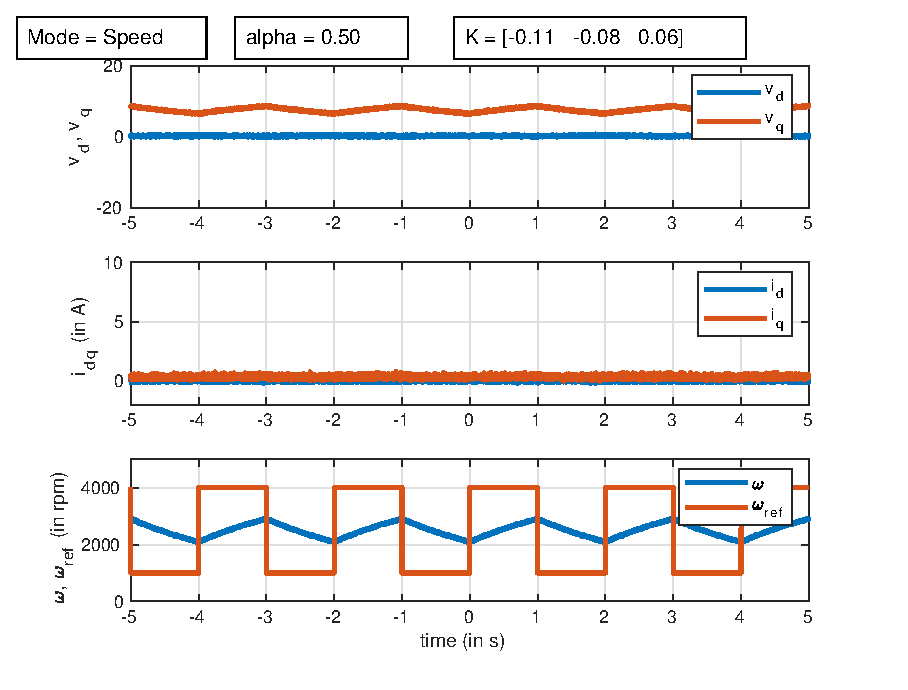
\includegraphics[width=0.7\framewidth]{pictures/expeSolver/LMI1.eps}}
             \caption{Experimental validation for $\alpha = 0.5$}
\end{figure}   
    \end{column}
    \end{columns}
\end{frame}
% \begin{frame}{Embedded control synthesis}{Experimental validation}
%     \begin{figure}[H]
%   \centering
%   \centerline{\includegraphics[width=0.7\framewidth]{pictures/expeSolver/LMI3.eps}}
%   \caption{Experiment validation for $\alpha = 5.80$.}
%   \label{fig:alpha5}
% \end{figure}
% \end{frame}

% \begin{frame}{Embedded control synthesis}{Experimental validation}
%     \begin{figure}[H]
%   \centering
%   \centerline{\includegraphics[width=0.7\framewidth]{pictures/expeSolver/LMI4.eps}}
%   \caption{Experiment validation for $\alpha = 25.87$}
%   \label{fig:alpha25}
% \end{figure}
% \end{frame}

\begin{frame}{Embedded control synthesis}{Experimental validation (no load)}
        \begin{columns}
        \begin{column}{0.4\textwidth}
            \begin{tikzpicture}[scale=1.5]
    \def\xmin{-1.4cm} \def\xmax{0.5cm}
    \def\ymin{-1.4cm} \def\ymax{1cm}

    \draw [thick,->] (\xmin,0) -- (\xmax,0) node [anchor = west]{\tiny $\operatorname{Re}$};
    \draw [thick,->] (0,\ymin) -- (0,\ymax) node [anchor = south]{\tiny $\operatorname{Im}$};
    \begin{scope}
      \clip (-1cm,-1cm) rectangle (-0.3cm,1cm);
      \fill[gray!30,opacity=0.6] (-0.3cm,0.3cm) -- (-0.3cm,-0.3cm) -- (-1cm,-1cm) -- (-1cm,1cm) -- cycle;
    \end{scope}
    \draw [darkGreen,line width= 0.3mm] (-0.3cm,-0.3cm) -- (-0.3cm,0.3cm);
    \draw [darkGreen,line width= 0.3mm,dashed] (-0.3cm,0.3cm) -- (-0.3cm,1cm);
    \draw [darkGreen,line width= 0.3mm,dashed] (-0.3cm,-0.3cm) -- (-0.3cm,-1cm);
    \draw [darkBlue,line width= 0.3mm, dashed] (0cm,0cm) -- (-0.3cm,0.3cm);
    \draw [darkBlue,line width= 0.3mm] (-0.3cm,0.3cm) -- (-1cm,1cm);
    \draw [darkBlue,line width= 0.3mm, dashed] (0cm,0cm) -- (-0.3cm,-0.3cm);
    \draw [darkBlue,line width= 0.3mm] (-0.3cm,-0.3cm) -- (-1cm,-1cm);
    % Add labels
    \draw[->,darkBlue] (-0.15,0.15) arc[start angle=145, end angle=175, radius=0.25cm];
    \node[text=darkBlue] at (-0.25,0.15) {\tiny $\psi$};
    \draw[<->,darkGreen] (-0.05,-0.9cm) -- (-0.25cm,-0.9cm) node[midway, below, text=darkGreen] {\tiny $\alpha$};
    \node[text=darkBlue] at (-1cm,1cm) [above left] {\tiny $\beta$};
    % Arrow pointing to the gray region from the left
    \draw [->,red,line width=0.4mm] (-1.3cm,0.5cm) -- (-0.6cm,0cm);
    \node[text=red,align=center] at (-1.6cm,0.8cm) {\tiny Minimize\\[-0.05cm]\tiny performance\\[-0.05cm]\tiny criterion};
    \end{tikzpicture}
    \end{column}
    
    \begin{column}{0.6\textwidth}
    
    \begin{figure}[H]
  \centering
  \centerline{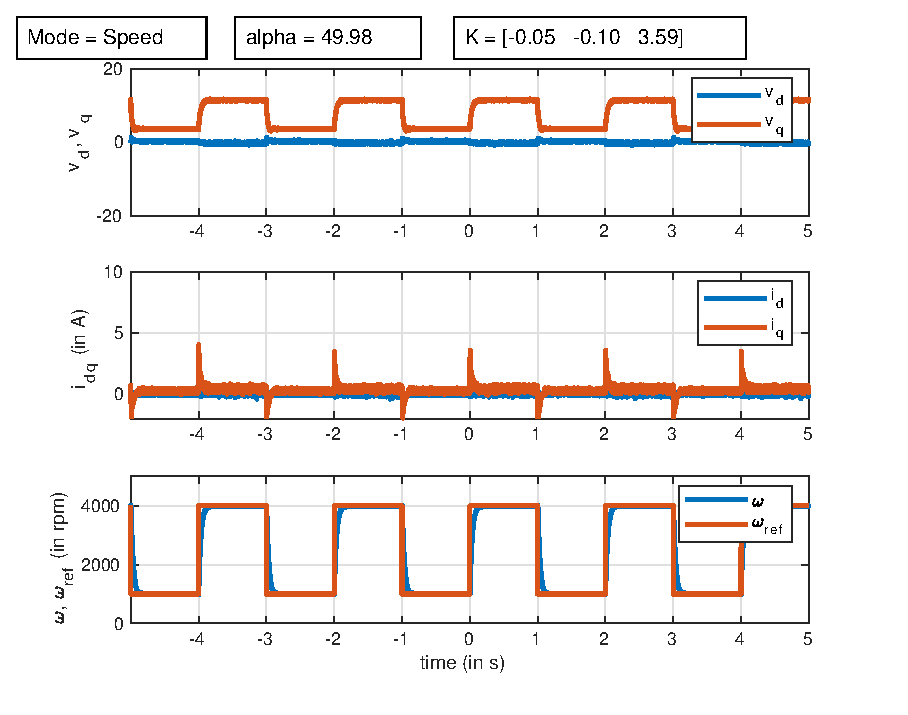
\includegraphics[width=0.7\framewidth]{pictures/expeSolver/LMI5.eps}}
  \caption{Experimental validation for $\alpha = 49.98$}
  \label{fig:alpha50}
  \end{figure}
    \end{column}
\end{columns}

\end{frame}

\begin{frame}{Embedded control synthesis}{Control performance: Results summary}
    \textbf{Experimental validation confirms:}

    \vspace{0.3cm}
    \begin{itemize}
        \item[$\checkmark$] \textbf{Solver operates correctly as idle task}
         \item[$\checkmark$] \textbf{No need for external intervention}

        \item[$\checkmark$] \textbf{Computational time for this application is 0.3 s}
        \begin{itemize}
            \item Dependent on the hardware, the size of the problem, or on the low priority task load.
        \end{itemize}
    \end{itemize}
    \vspace{+0.1cm}
    \textbf{Remark:}
    \begin{itemize}
        \item the LMI solver is generic
    \end{itemize} 

    \vspace{0.3cm}
    \begin{center}
    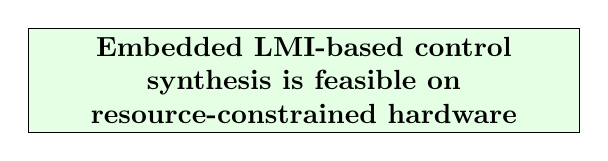
\begin{tikzpicture}
        \node[draw, rectangle, fill=green!10, minimum width=7cm, minimum height=0.8cm] {
            \begin{minipage}{6.5cm}
                \centering
                \textbf{Embedded LMI-based control synthesis is feasible on resource-constrained hardware}
            \end{minipage}
        };
    \end{tikzpicture}
    \end{center}
\end{frame}



%%%%%%%%%%%%%%%%%%%%%%%%%%%%%%%%%%%%%%%%%%%%%%%%%%%%%%%%%%%%%%%%%%%%%%%%%%
\begin{frame}{Outline}
        \textbf{Objectives:}
    \vspace{0.2cm}
    \begin{enumerate}
        \item[\textcolor{darkgray}{\textbf{1.}}] \textcolor{darkgray}{\textbf{What are the optimal currents $i_d^\#$, $i_q^\#$ to produce desired torque $\tau$ and speed $\omega$ ?}}
        \item[\textcolor{darkgray}{\textbf{2.}}] \textcolor{darkgray}{\textbf{Embedded closed-loop control synthesis}}
        \item[\textcolor{Blue4}{\textbf{3.}}] \textcolor{Blue4}{\textbf{New control approaches}}
    \end{enumerate}
        \begin{figure}
            \begin{center}
                \def\textsize{.8}
                \psfrag{Algo}[c][c][1]{\color{Blue4}Control}
                \psfrag{Control}[c][c][1]{\color{Blue4}Control}
                \psfrag{iabc}[c][c][\textsize]{\color{Blue4}$i_{abc}$}
                \psfrag{idq}[c][c][\textsize]{\color{Blue4}$i_{dq}$}
                \psfrag{vabcr}[c][c][\textsize]{\color{Blue4}$v_{abc}^\#$}
                \psfrag{vdqr}[c][c][\textsize]{\color{Blue4}$v_{dq}^\#$}
                \psfrag{dq}[c][c][.5]{\color{Blue4}${dq}$}
                \psfrag{abc}[c][c][.5]{\color{Blue4}${abc}\quad$}
                \psfrag{S}[c][c][\textsize]{\color{Blue4}$S_{abc}$}
                \psfrag{MLI}[c][c][\textsize]{\color{Blue4}Mod}
                \psfrag{ParkInv}[c][c][.5]{}
                \psfrag{Park}[c][c][.5]{}
                \psfrag{TS1}[l][c][.6]{\color{Blue4}Higher priority $\approx20$kHz}
                % Reference generation (cyan) - lower priority optimization
                \psfrag{Vr}[c][c][\textsize]{\color{Cyan4}$\rho^\#$}
                \psfrag{ref}[c][c][\textsize]{\color{gray}$\omega^\#$}
                \psfrag{ref2}[c][c][\textsize]{\color{gray}$i_d^\#$}
                \psfrag{ref3}[c][c][\textsize]{\color{gray}$\omega^\#$}
                \psfrag{ref4}[c][c][\textsize]{\color{Cyan4}$i_q$}
                \psfrag{ref5}[c][c][\textsize]{\color{gray} Specification}
                \psfrag{ref6}[c][c][\textsize]{\color{gray} Model}
                \psfrag{Reference}[c][c][\textsize]{\color{gray}Trajectory}
                \psfrag{calculation}[c][c][\textsize]{\color{gray}generation}
                \psfrag{TS2}[l][c][.6]{\color{Cyan4}Lower priority $\approx1$kHz}
                % Embedded synthesis (magenta) - idle task
                \psfrag{Emb}[c][c][\textsize]{\color{gray}Embedded}
                \psfrag{Synt}[c][c][\textsize]{\color{gray}synthesis}
                \psfrag{K}[c][c][\textsize]{\color{gray}K}
                \psfrag{TS3}[l][c][.6]{\color{Magenta4}Idle task}
                % Physical system (red) - PMSM and measurements
                \psfrag{Onduleur}[c][c][\textsize]{\color{Red4}Inverter}
                \psfrag{PMSM}[c][c][\textsize]{\color{Red4}PMSM}
                \psfrag{V}[c][c][\textsize]{\color{Red4}$v_{abc}$}
                \psfrag{th}[c][c][\textsize]{\color{Red4}$\theta$}
                \psfrag{w}[c][c][\textsize]{\color{Red4}$\omega$}
                \psfrag{thm}[c][c][\textsize]{\color{Red4}$\theta$}
                \psfrag{wm}[c][c][\textsize]{\color{Red4}$\omega$}
                \psfrag{Embedded}[l][c][.7]{\color{red}Embedded code}
                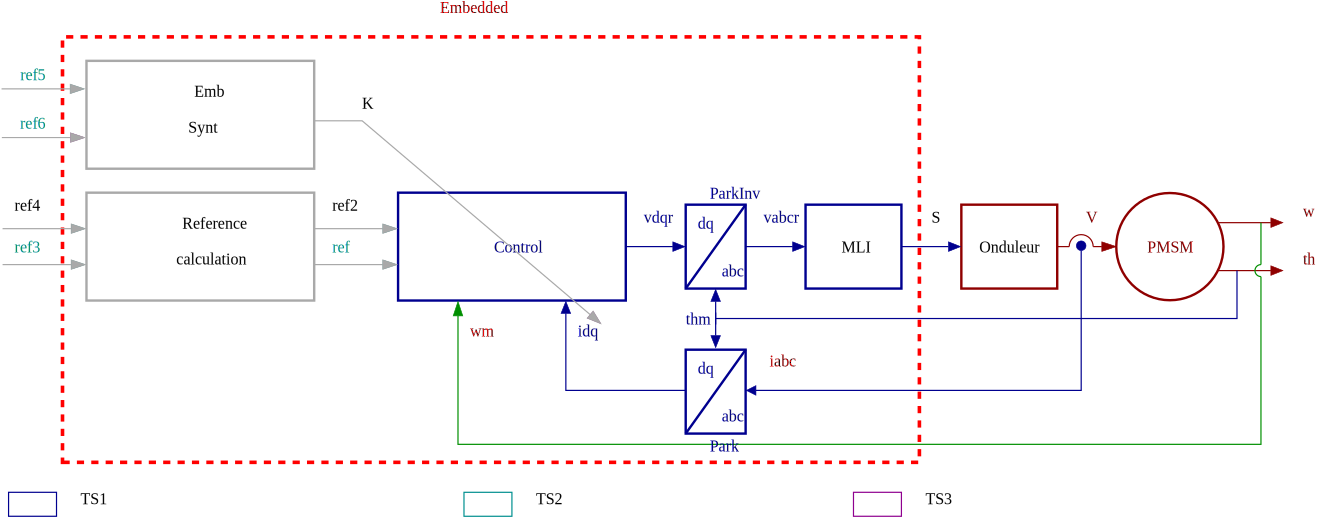
\includegraphics[width = .9\textwidth]{pictures/AdvancedControl_control.eps}
            \end{center}
        \label{fig:AdvencedControlForElectricalMotor}
        \end{figure}
\end{frame}

